\documentclass[lettersize,journal]{IEEEtran}
\usepackage{amsmath,amsfonts}
\usepackage{algorithmic}
\usepackage{algorithm}
\usepackage{array}
\usepackage[caption=false,font=normalsize,labelfont=sf,textfont=sf]{subfig}
\usepackage{textcomp}
\usepackage{stfloats}
\usepackage{url}
\usepackage{verbatim}
\usepackage{graphicx}
\usepackage{cite}
\hyphenation{op-tical net-works semi-conduc-tor IEEE-Xplore}
%\usepackage{tikz,graphics,color,fullpage,float,epsf,caption}
% updated with editorial comments 8/9/2021

\begin{document}

\title{The Risks and Benefits of Social Media, and Its Place in Higher Education: a study}

\author{Daniel T. Daley,~\IEEEmembership{Falmouth University}}
        % <-this % stops a space


%\thanks{This paper was produced by the IEEE Publication Technology Group. They are in Piscataway, NJ.}
% <-this % stops a space
%\thanks{Manuscript received April 19, 2021; revised August 16, 2021.}

% The paper headers
%\markboth{Journal of \LaTeX\ Class Files,~Vol.~14, No.~8, August~2021}
%{Shell \MakeLowercase{\textit{et al.}}: A Sample Article Using IEEEtran.cls for IEEE Journal
%\IEEEpubid{0000--0000/00\$00.00~\copyright~2021 IEEE}

% Remember, if you use this you must call \IEEEpubidadjcol in the second
% column for its text to clear the IEEEpubid mark.
\maketitle
\begin{abstract}
	This study investigates how students have performed when exposed to social media in
	a learning context to facilitate the development of an institutionalised social media platform for
	universities. I will conduct a literature review covering three areas, 'Social media in higher education'
	to gauge the effectiveness of student engagement, 'The effects of social' media to explore any potential
	risks in an effort to build the platform both ethically and responsibly, and finally user interface and
	user experience patterns of social media. I hypothesize that an institutionalised social media platform
	could be a benefit to students by easing their onboarding process by a better space to find their cohort,
	and academically by making course related materials more accessible in a familiar feeling domain. 
\end{abstract}

\begin{IEEEkeywords}
Social Media, Social Networking, Higher Education.
\end{IEEEkeywords}

\section{Introduction}
	Social media is all around us, and the vast majority of us use social in some way or another very
	frequently. Many studies have taken place to explore the impact social media could have on students
	when they have been encouraged to use existing platforms as a contact and collaboration tool as part
	of their course. 
    Finding your place socially at university can be very daunting, especially if you have been unable to find
    your way into any large social events, or onto any student-run social channels such as Discord etc, if any
    such things are in place at all. Failure to find such places can have a major impact on not only the university
    experience but also their mental health, as they can find themselves isolated. I plan to research into the
    question; could a social media platform embedded into higher education institutions be of benefit to students
    starting university by aiding their integration into their new social setting?

\section{Related Work}
    This literature review investigates the risks and benefits attached to
    social media and the potential advantages that it could bring forward as a
    tool in higher education and pedagogy. Social media has made a massive
    impact on society in many ways, and using it one way or another has become
    commonplace in most of our lives, but do we fully understand the risks and
    advantages that it presents? This literary analysis of recent (2010-2022)
    research papers aim to explore findings on the possible side effects of
    social media in an effort to weigh the pros against the cons regarding
    the integration of social media with higher education (HE) and pedagogy. I
    hypothesize, that with proper application, social media could become a valuable
    tool within HE institutions and could help increase engagement with learning
    materials and courses.
\subsection{Social Media in Higher Education}
    Liu \cite{Liu2010}  acknowledges that each social media platform comes with
    its own set of strengths and weaknesses and that the integration of such into
    pedagogy must be planned cautiously, ensuring that it is the strengths of the platform
    that are leveraged and not the potential distractions and difficulties that could
    hinder student learning. Liu talks of each social media platform being a tool,
    each in its own specific right and each with its designated purpose, so a one size
    fits all approach would only bring about nuisance. The author notes, for instance,
    that we could capitalize on Facebook's ubiquity and capabilities for collaboration.
    Liu \cite{Liu2010} and Baruah \cite{Baruah2012} both talk about the integration of
    social media into higher education and both conclude by sharing their thought on that
    it would be an advantage to implement social media elements as tools within higher
    education. Baruah further empowers Liu's point about different platforms providing
    different tools, by discussing how much easier collaboration becomes when using
    online facilities. Online mediums that provide features allowing users to co-draft
    documents, organize members, arrange meetings, spread information, and gauge opinion,
    all while having the capability to reach audiences all over the world.
    Baruah concludes that there will be a greater capacity for groups to participate in
    collective action, going on to say that it is the hallmark of civil society.

    Kelm \cite{Kelm2011} also implemented social media into their course and noticed an
    increase in engagement from their students and reported a greater sense of team ethic
    between classmates. Kelm concluded with a note stating that the secret for educators is
    to observe how technology is used in everyday life and then implement that use into
    our education systems.
    Wang et al. \cite{Wang2011} mention in their paper that there is a call for an approach
    to try and better balance the relationship between social media and academic study but
    pays a great deal of respect to the potential benefits that it can offer. The paper goes
    on to mention that students are very likely to be affected by social media, whilst it
    provides a world in which to make new friends and release pressure, it can absolutely
    impact students' lives and grades, calling for the aforementioned balance.

    Evans \cite{Evans2014} encouraged students to interact with him and their peers through
    Twitter and found that the amount of Twitter usage was associated with increased student
    engagement. Course-related tweeting showed no evidence of being related to interpersonal
    relations between students and their tutors, and finally that Twitter usage did not relate
    to class attendance.

    Williams \cite{Williams2022} talks of the capabilities that social media brings
    forward as advantages in enhancing learner engagement in a very efficient way
    and reiterates the points provided by Junco et al \cite{Junco et al 2013}.
    The paper from Junco et al. follows a similar experiment to Evans and his 2014
    paper \cite{Evans2014} but in a slightly more robust and comprehensive fashion.
    This was achieved by using two separate groups, the first consisting of 125
    students, half of whom were required to use Twitter while the other half were
    required to use Ning, whereas the participation of Twitter and Ning usage was
    voluntary for study group 2. The study recognised greater motivation towards
    engagement from study group 1 (those required to use Twitter and Ning). The
    paper concludes by stating that new technologies being incorporated into contemporary
    classrooms is an important development in an effort to produce more effective
    learning strategies and outcomes, while calling for contemporary students to
    improve their capacity to engage in more self-directed collaborative practices
    in order to better take ownership of their learning.

    Tripathi \cite{Tripathi 2022} observed that nearly two-thirds of faculty at
    their institution had used social media in a class session, some even
    posting content for students to further read outside of classes, which saw
    promising levels of engagement while other members of the faculty ask students
    explicitly to utilise social media as part of course assignments. On an end
    note the paper reaffirms that the presence of social media within HE is
    increasingly visible as instructors continue to further employ technology
    to enhance their teaching methods and promote active learning for students.

    Haythornthwaite, Paulin, and Gruzd \cite{Haythornthwaite et al 2016}  discuss
    an overview of the measures and potential of a multi-method approach for studying learning
    through means of social media, based on a workshop held at the 2014 Learning
    Analytics and Knowledge conference. The paper pays vast respect to the
    implementation of social media into both teaching and learning being new,
    but still advancing rapidly. It is recognised that learners are already
    present on these channels and are already capable of information search and
    acquisition, learning community support, knowledge building, and engagement.
    In one of the final notes of the paper, there is mention that different
    settings of formality would call for different considerations to be made. In
    a formal setting, the intent of the instructor must be taken into
    consideration while examining the discussion formation comparatively against
    the desired communication and pedagogical outcomes. Whereas in more informal
    settings, we must consider the impact of things on a more societal level of
    mass learning and how the balance of the development of sustained learning
    communities is affected by massively distributed learning and the
    'just-in-time learning' associated with social media exchanges.

\subsection{The Effects of Social Media}
    The paper by Amedie \cite{Amedie 2015} mentions that, ironically, social
    media is in effect turning us into one of the most antisocial generations
    yet. The paper talks about the connection between social media and anxiety
    – It states that social media causes depression and anxiety in two ways. Chronic
    stress causes depression and anxiety. Being constantly alert for new social
    media messages, to your instinctive fight or flight limbic system, is the
    same as being on continuous alert for predators, which causes a release of
    the stress hormone cortisol. The second cause of depression anxiety is
    constantly trying to maintain an unrealistic and unachievable image of
    oneself on their chosen social network. The paper also mentions
    that social media can pave the way for criminal activity, by putting to use
    the freedoms offered by social media to hide their identity and engage in
    things like cyberbullying, cyber terrorism, human trafficking and drug dealing,
    though only talks in depth of cyberbullying, criminal and terrorist activities
    as they are the most common illicit activities. Amedie concludes that despite
    the positive benefit of rapid information sharing, social media enables people
    to create false identities and superficial connections, causes depression and
    is a primary recruiting tool for criminals and terrorists. It also mentions
    that the negative impacts of social media are rarely discussed, while the benefits
    are often emphasized.

    Kuppuswamy and Narayan \cite{Kuppuswamy et al 2010} recognise that social
    media sites provide function for individuals to create and maintain social
    ties, which can be of a great benefit in both academic and social settings.
    It is also observed that these same sites present risk to individuals'
    privacy, health, safety and professional reputations if the platforms are
    not used responsibly.

    In a 2012 paper by Tariq et al \cite{Tariq et al 2012}, the authors observed that more than 90\%
    of college students use social media \cite{Ellison et al 2007} and they found social media to be
    having a negative impact on education. Tariq et al believe this to be due to social networks
    capturing the total attention of its users and redirecting them towards non-educational, innapropriate
    and unnethical activities such as 'useless chatting, time killing by random searching and not doing their jobs'. The paper
    goes on to note that social networking sites quite often play host to attractive activities such
    as gaming or advertisements, enticing people to sign up or simply waste time, it is the over-indulgeance
    of such activities that cause users to develop social media addiction. It states that providing ubiquitous
    facility of social networks is a straight invititation of addiction to any teenager and even an adult, as
    academic satisfaction is not enough got those students who suffer from social isolation\cite{Pempek et al 2009}.   

    A study conducted by W.Akram and R.Kumar \cite{Akram et al 2017} observes the both the negative
    and positive impacts of social media on society and business.  The paper notes the merits presented by social media
    while also recognising that it has some faults. Touching on social media within higher education, Akram et al
    discuss that social media allowing individuals to share thoughts with others on the other side of the planet instantly
    is a massive positive, and in many cases this shared information then becomes easily available for many others to
    see and benefit from. The literature saw that social media helped in development towards simply being more prepared, stating that
    social media is fundamentally about showcasing and taking part in  current trends around the world, futher enabling students
    to plan or guage an idea of what might be expected of them. In contrast of those points, the paper outlines that
    social media could aid toward reduced learning and research capabilities. With a growing dependency on information
    being easy to find, this could hinder the development of research skills. In most cases people tend to use slang or
    abbreviated language on social media as most relationships between individuals tend to be interpersonal, coupled
    with an increased reliance on spellcheckers and autocorrection, this decreases their charge over the dialect and
    formal writing abilities. Another valuable note from the paper shines light on time wastage, while social media
    and the internet in general are a boon for education, it opens the door for many distractions if the right amount
    of self-discipline is not present. While social networking has improved the quality and rate of coordinated
    efforts from students, it remains important to be responsible and understand the possible negative effects
    that social media brings forward. A general consensus is established with Tariq et al's \cite{Tariq et al 2012}
    points on the factor of distraction before concluding that people are advised to adopt the positive aspects of
    social media while avoiding the negatives, in an effort to benefit from the latest and emerging technologies.

    Kaur and Bashir \cite{Bashir et al 2015} reiterate that there are many benefits to social media use
    for adolescents, and that there are also multiple potential risks that can act in detriment to their
    mental health and well-being. Some of the positive impacts outlined were access to health information,
    enhanced communication and learning opportunities, while the negatives involve stress, depression,
    suppression of emotional awareness, fatigue, online harassment, decline of intellectual ability
    and a shrinking capacity for concentration. The paper goes on to express that these risks could be
    navigated successfully with proper handling, such would call for an education around social media abuse
    being provided (expressly to parents to mitigate the risks for children and adolescents), but a greater
    awareness of the capacity for potential harmful effects that these platforms can inflict must be attained.

    Bashir and Bhat \cite{Bashir et al 2017} touch on these points again exploring the psychological effects
    of social media, asserting that excessive use of social media can lead people to disastrous results, starting
    with anxiety and leading to depression. They saw in Pantic et al.'s study \cite{Pantic et al 2012}, mirrored
    by a study conducted by Rosen et al. \cite{Rosen et al 2013}, that depression and time spent on Facebook by
    adolescents were directly correlated and that those that spent most of their time engaging in online activities
    were among those with major depressive symptoms. The paper concludes to suggest that social media can have an
    epidemic-like on any individual. Social networking sites should be constrained to an age limit and that any
    social media application that does not have a positive impact and enables such things as discrimination, violence
    and racism should be dissolved at once, completely.

    Naslund et al. \cite{Naslund et al 2020} found in their paper that in young people, many benefits to social
    media were recognised. Among these benefits were elevated self-esteem and more opportunities for self
    disclosure. Some of the negative aspects observed were an increased exposure to harm, depressive symptoms,
    social isolation and bullying. The paper concludes highlighting that social media has become an important part
    of the lives of many individuals living with mental disorders, and that many of which use social media to share
    lived experiences regarding mental illness, seek support from others, find treatments and recommendations as
    well as access to mental health services. It also recognises that social media platforms could be used to
    allow individuals to access evidence based treatments and support. The authors end on the recognition that to
    fully close the gap in mental health services integrated into social media, that it would require researchers
    to work closely with clinicians to make sure that benefits of such things on social media platforms would
    out-weigh any possible risks.
\section{Evaluation}

	\subsection{Social Media in higher Education}
	Almost all papers found positive outcomes with integrating social media into higher education and in most cases the utility and ease
	of collaboration is at the center of praise. It is recognised that each platform has something different to offer and we are perhaps 
	better off to see them as tools each in their own regard, built for their own purpose. With that said, one characteristic shared among these platforms
	 is the opportunity to easily reach others from across the globe whilst still making effective team management and organization possible and instant.
	 The studies observed noted an increase in team ethic with the introduction of social media in their courses and a direct correlation between
	 social media usage and course engagement while their online activities showed no evidence of being related to interpersonal relationships
	 between students and their tutors. Another consensus is that to fully leverage social media within higher education, a balance must be found.
	 Social media sites play host to many distractions and irrelevant activities and nonesensical information, calling for responsibility of domain
	 selection, and responsility of proper use. In the same vein as striking balance, setting and formality must be taken into consideration, different
	 approaches and rule sets may need to be applied between settings of different formality and would not be a one size fits all scenario. To fully 
	 employ social media into pedagogy, the staff and faculty would be at the heart of operations, it would require a small degree of technical competence and
	 familiarity for teaching staff to use such platforms effectively and engagingly.
	 All literature reviewed conducts a study on existing mediums of social media where distractions already exist and the courses may have altered slightly  to
	 fit into social media space. For this research project I will build a platform expressly for use within higher education,
	 and conduct my study in the same fashion as those previously mentioned.

	\subsection{Effects of social media}
	All studies reviewed seem to agree that there is a need for a greater understanding of the risks of social media in order to fully
	 be able to leverage its many benefits. Social media sites if left unmonitored can be the prime environment for negative things to thrive 
	 such as bullying and discrimination. There is also the less directly harmful aspects to consider, such as excessive amounts of advertisements that 
	 cause distraction and promote time wasting and other non-productive activities. It is engaging in these activities and succumbing to the lure of
	 these advertisements that gives social media its addictive nature, which if left unchecked can lead to conditions such as depression and anxiety.
	 To satisfy the concerns outlined by the literature, a platform would need to be created with these points at the forefront of its design.
	 It would need to be engaging but not distracting, a place safe from harm and free from discrimination and bullying, and host activities on
	 which time spent is time well spent\section{Proposed Research}
	\subsection{Question}
	Research question stuff goes here.

	\subsection{Hypothesis}
	Expected outcome goes here.

	 I hypothesize that an institutionalised social media platform
	could be a benefit to students by easing their onboarding process by a better space to find their cohort,
	and academically by making course related materials more accessible in a familiar feeling domain. 
\section{Research Methodology}

	\subsection{Philosophical Position}
	Having great applications within sociology and psychology, the philosophical approach of this study will be from an 
	interpretivist point as the application of this platform and the observations of its utility align with the social
	 sciences and as such will require a socioscientific approach. This interpretivist approach by its nature calls for a qualitative
	 method; often criticised for its generalisability and flaws in reliability, I will combine quantitative and qualitative methods
	 in order to increase reliability and validity of findings through means of triangulation.

    	\subsection{Experimental Design}
    	To gather information on the effectiveness of my platform, I will conduct a between groups study involving
    	two study groups. Both groups will be given the same set of tasks to complete, group A will be asked to fulfil 
    	these tasks on the existing online university portal ie Learning Space or Moodle while group B will
	do so on the prototype platform. I will use a survey to collect information on the test users experiences
    	of both platforms in an effort to gauge how much of a benefit they feel the systems offer in both the
    	learning and social aspects of university life. The survey will be conducted in a similar manner to
	studies explored in the review of literature \cite{Liu2010}\cite{Baruah2012}\cite{Wang2011}\cite{Evans2014}\cite{Akram et al 2017},
	the results obtained from those papers seem proficient and I feel it well justifies the survey as a means for collecting data.
	We have chosen a between subjects study	as each group will be testing only one platform as a cohort and asked to test all functionalities of
    	the system as per the tasks.

	\subsection{Data Management Plan}
	Data management plan stuff here
LOGISTICAL REGERESSION R CODE SURVEY
	\subsection{Validation and Verification}
	How will I acheive validation and verification of my findings

	\subsection{Ethical Considerations}
	Given the nature of this research and given that there will be participants studied...

\section{Artefact Design}

	The title of platform is ``myUniSocial", the core of which will be an evolution of my work carried out in developing a previous social media system \cite{Daley 2022}.
	The previous system or `myCircle'\cite{myCircle} is built around interests and hobbies as opposed to simple media reposting in an
	effort to navigate the negative impacts observed in the above review of literature and the comparison culture that exists in modern
	society. In recognition of the distraction factor mentioned by many in the literature review, it feels like somewhat of a responsibility
	to minimise possible distractions on the platform, and if they do exist, to make them a benefit to engage with and for it to be relevant
	to their course. To acheive this, in place of of the interest groups or `circles', course modules could be displayed allowing users to
	quickly access course content and helpful materials. Work from my other
    platform `myUni404' \cite{myUni404} will be built in as a feature to aid students
	on various fields of computing, this platform offers users the ability to post coding and programming questions, and is browsable by speciality
	ie. -  Web Development, Game Development, Robotics and so on. `myUni404' is built with a beginner friendly focus and this will be a great
	step in the direction of making the social network educational while building confidence in expertise.


	\begin{figure}[h!]
		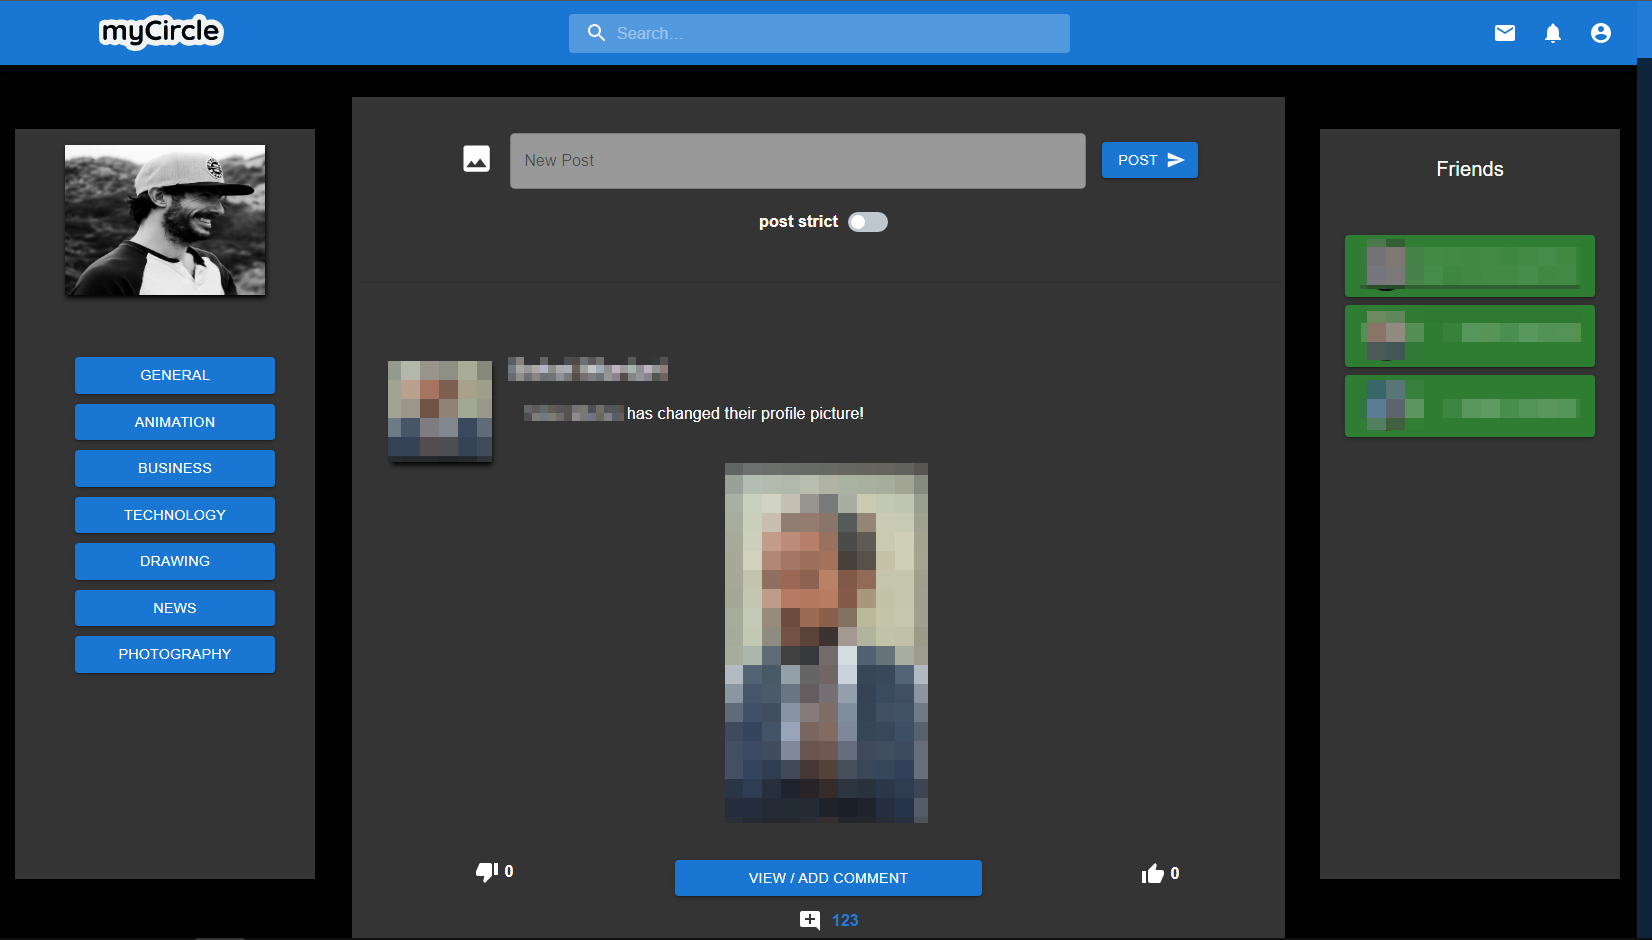
\includegraphics[width=\linewidth]{myCircle.PNG}
		\caption{myCircle user interface}
		\label{figure 1}
	\end{figure}


	In appendix A figure 1 we can see a class diagram for the base system, with main functionality coming from 'App.js' and being passed into
	functional child components. This class diagram is a derviative of the previously mentioned 'myCircle' system with the relavant adjustments,
	as is the same for the Use Case Diagram which can be seen at Appendix A figure 2.

	\subsection{Technological Stack}
	The stack for this platform will be a React.js front end \cite{React} making use of Material UI for styling \cite{Mui}, alongside a Node powered back end \cite{Node} with Express for server functionality\cite{Express} . 
	How will I get around the issues summarised in the literature review.
	\subsection{Testing of artefact performance}
	How will I test the performance of my aretefect.


%\section*{Acknowledgments}
 %   This should be a simple paragraph before the References to thank those individuals and
 %   institutions who have supported your work on this article.


%{\appendices
%\section*{Proof of the First Zonklar Equation}
%Appendix one text goes here.
% You can choose not to have a title for an appendix if you want by leaving the argument blank
%\section*{Proof of the Second Zonklar Equation}
%Appendix two text goes here.}



%\section{References Section}
%You can use a bibliography generated by BibTeX as a .bbl file.
% BibTeX documentation can be easily obtained at:
% http://mirror.ctan.org/biblio/bibtex/contrib/doc/
% The IEEEtran BibTeX style support page is:
% http://www.michaelshell.org/tex/ieeetran/bibtex/
%
 % argument is your BibTeX string definitions and bibliography database(s)
%\bibliography{IEEEabrv,../bib/paper}
%
%\section{Simple References}
%You can manually copy in the resultant .bbl file and set second argument of $\backslash${\tt{begin}} to the number of references
% (used to reserve space for the reference number labels box).

\begin{thebibliography}{}
\bibliographystyle{IEEEtran}

\bibitem{Liu2010}
        Liu, Youmei {\it{Social Media Tools as a Learning Resource}} Journal of Educational Technology Development and Exchange (JETDE): Vol. 3 : Iss. 1, Article 8, 2010

\bibitem{Baruah2012}
    Baruah, Trisha Dowerah {\it{Effectiveness of Social Media As a Tool Of Communication And Its Potential For Technology Enables Connections: A Study.}}, New York, NY, USA: Springer, 2007.

\bibitem{Kelm2011}
    Kelm, Orland R. {\it{Social Media: It's What Students Do.}}Business Communication Quarterly, Volume 74, Number 4, December 2011.

\bibitem{Wang2011}
        Wang, Qingya / Chen, Wei / Liang, Yu {\it{The Effects of Social Media on College Students}}.MBA Student Scholarship, Paper 5. 2011.
\bibitem{Evans2014}
        Evans, C. {\it{Twitter for Teaching: Can Social Media Be Used To Enhance The Process Of Learning?}} British Journal of Education Technology
Vol 45, No 5, 2014.

\bibitem{Williams2022}
        Williams, R. Thomas {\it{Social Networking Services (SNS) In Education}}
        Asian Journal of advances in Research. 17(1): 1-4, 2022.

\bibitem{Junco et al 2013}
        Junco, R. / Elavsky, C. Michael / Heiberger, G. {\it{Putting Twitter to
        the test: Assessing outcomes for student collaboration, engagement and
        success.}} British journal of Education Technology. Vol 44 No 2 2013

 \bibitem{Tripathi 2022}
        Tripathi, Dr. Sheel Nidhi {\it{Social Media in Higher Education}}
        Communication Today, January-June, 2022.

\bibitem{Haythornthwaite et al 2016}
    Haythornthwaite, C. / Paulin, D. / Gruzd, A. {\it{Analyzing Social Media
        and Learning Through Content and Social Network Analysis: A Faceted
        Methodological Approach.}} Journal of Learning Analytics, 3(3), 47-71.
        2016.
\bibitem{Amedie 2015}
        Amedie, J. {\it{The Impact of Social Media on Society.}}
        Advanced Writing: Pop Culture Intersections. 2
        2015.
\bibitem{Kuppuswamy et al 2010}
	Kuppuswamy, S /Shankar Narayan, P. B. {\it{The Impact of Social Networking Websites on the Education of Youth.}}
	International Journal of Virtual Communities and Social Networking, 2(1), 67-79.
	2010.
\bibitem{Tariq et al 2012}
	Tariq, W. / Mehboob, M. / Khan, M. Asfandyar / Ullah, F. {\it{The Impact of Social Media and Social Networks on Education and Students of Pakistan.}} International Journal of Computer Science Issues, Vol. 9, Issue 4, No 3.
	2012.
\bibitem{Ellison et al 2007}
	Ellison, N. / Steinfield, C. / Lampe, C. {\it{The Benefits of Facebook "friends:" Social Capital and College Students' Use of Online Social Network Sites.}} Journal of Computer-Mediated Communication, Vol 12, 4.
	2007.
\bibitem{Pempek et al 2009} 
	Pempek, Tiffany A / Yermolayeva, Yevdokiya A. / Calvert, Sandra L. {\it{College students’ social networking experiences on
		Facebook.}} Journal of Applied Developmental Psychology, Vol. 30, Issue 3, page 227–238.
	2009
\bibitem{Akram et al 2017}
	Akram, A. / Kumar, R. {\it{A Study on Positive and Negative Effects of Social Media on Society.}}
	International Journal of Computer Sciences and Engineering, Vol 5, 10.
	2017
\bibitem{Bashir et al 2015}
	Kaur, R. / Bashir, H. {\it{Impact of Social Media on Mental Health of Adolescents.}}
	International Journal of Education, 5, 22-29.
	2015
\bibitem{Bashir et al 2017}
	Bashir, H. / Bhat, S. A. {\it{Effects of Social Media on Mental Health: A Review}}
	The International Journal of Indian Psychology, Vol 4, Issue 3.
	2017
\bibitem{Pantic et al 2012}
	Pantic, I. / Damjanovic, A. / Todorovic, J. / Topalovic, D. / Bojovic-Jovic, D. / Ristic, S. Ristic/ Pantic, S.
	{\it{Association Between Online Social Networking and Depression in High School Students: Behavioural Physiology Viewpoint.}}
	Psychiatria Danubina, 24(1), 90-93.
	2012.
\bibitem{Rosen et al 2013}
	Rosen, L.D. / Whaling, K. / Rab, S. / Carrier, L.M. / Cheever, N.A.{\it{Is Facebook Creating "iDisorders"? The Link Between Clinical Symptoms of Psychiatric Disorders and Technology Use, Attitudes and Anxiety.}} Computers in Human Behaviour, 29, 1243-1254.
	2013.
\bibitem{Naslund et al 2020}
	Naslund, John A. / Bondre A. / Torous J. / Aschbrenner, Kelly A. {\it{Social Media and Mental Health: Benefits, Risks, and Opportunities for Research and Practice.}} Journal of Technology in Behavioral Science 5:245-257.
	2020.
\bibitem{Daley 2022}
	Daley, D. {\it{A Creative Approach to Social Media}}
\bibitem{myCircle}
	{\it{myCircle}}
	http://dd252935.kemeneth.net:9010/
\bibitem{myUni404}
    {\it{myUni404}}
    http://147.182.247.158:9010/
\bibitem{React}
	{\it{React JS}}
	https://reactjs.org/
\bibitem{Mui}
	{\it{Material UI}}
	https://mui.com
\bibitem{Node}
	{\it{Node JS}}
	https://nodejs.org
\bibitem{Express}
	{\it{Express JS}}
	https://expressjs.com
\end{thebibliography}
\newpage
\newpage
\clearpage
%{\appendix[Proof of the Zonklar Equations]
%    Use $\backslash${\tt{appendix}} if you have a single appendix:
%    Do not use $\backslash${\tt{section}} anymore after $\backslash${\tt{appendix}}, only $\backslash${\tt{section*}}.
%    If you have multiple appendixes use $\backslash${\tt{appendices}} then use $\backslash${\tt{section}} to start each appendix.
%You must declare a $\backslash${\tt{section}} before using any $\backslash${\tt{subsection}} or using $\backslash${\tt{label}} ($\backslash${\tt{appendices}} by itself
% starts a section numbered zero.)}
\appendices
\newpage
\section{UML Diagram}

\begin{figure}[h!]
	\begin{tabular}{@{}c@{}}
		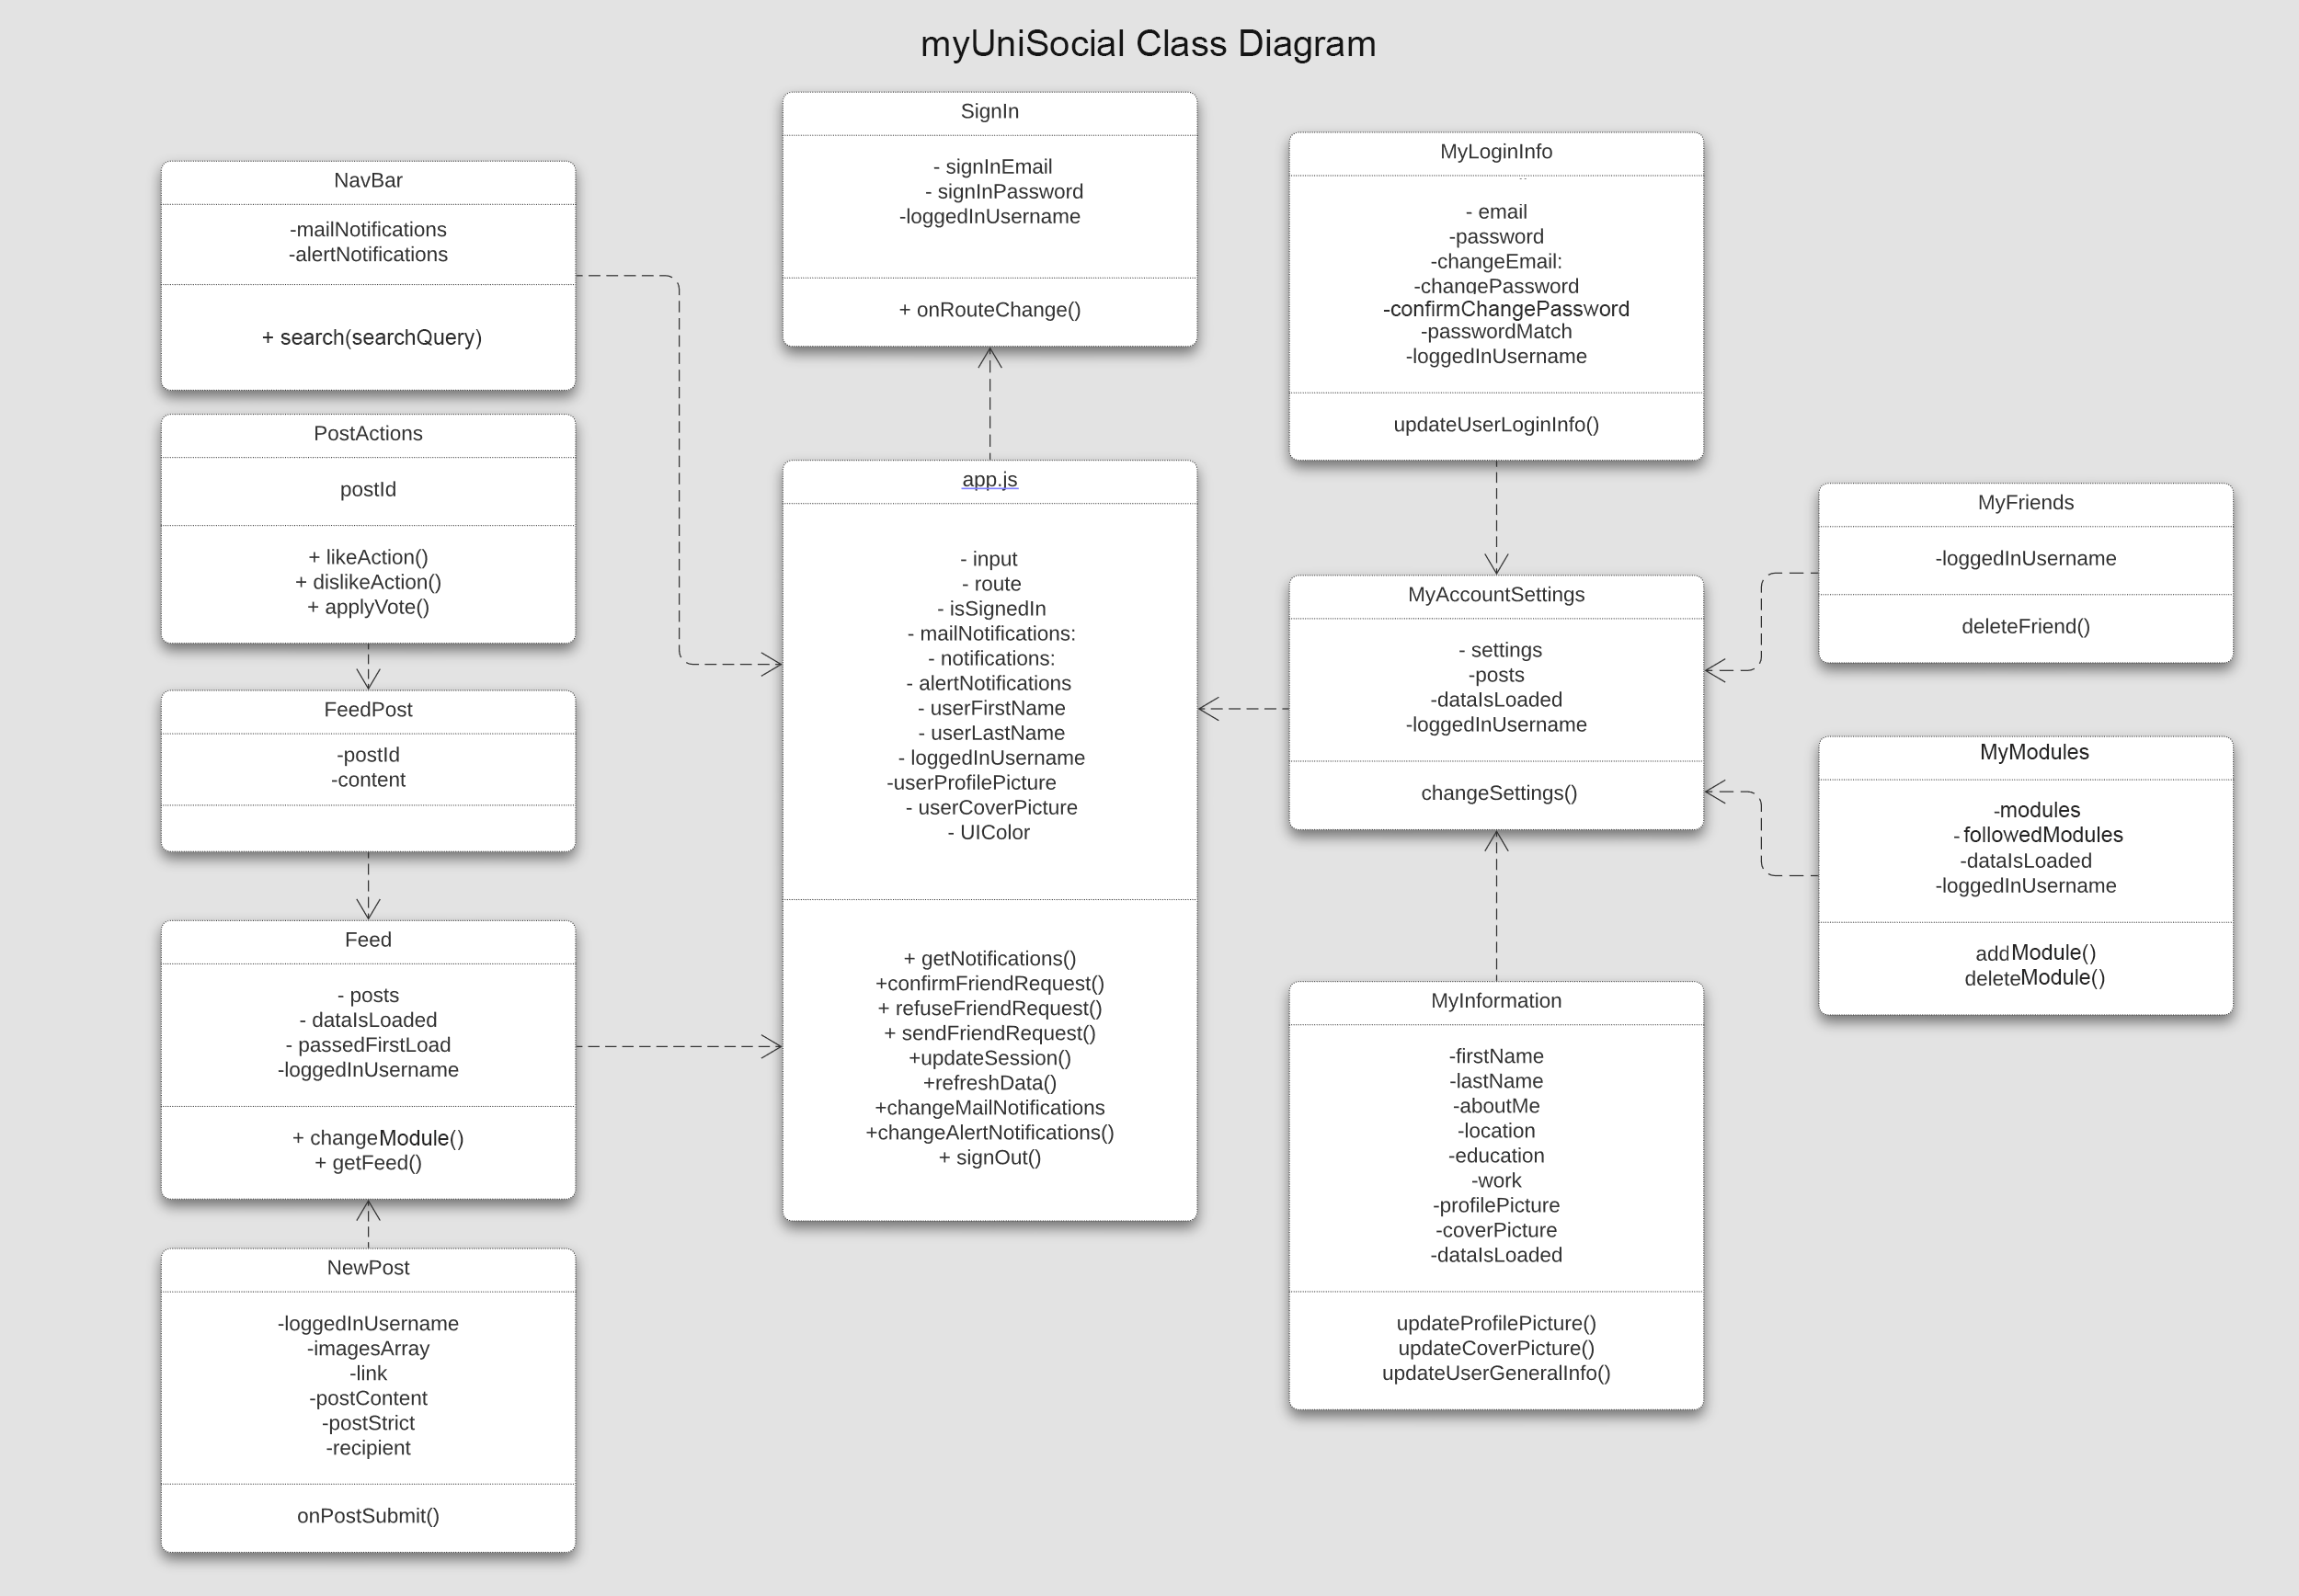
\includegraphics[width=.8\textwidth]{myUniSocialClassDiagram.png}
  	\end{tabular}



 	\begin{tabular}{@{}c@{}}
 		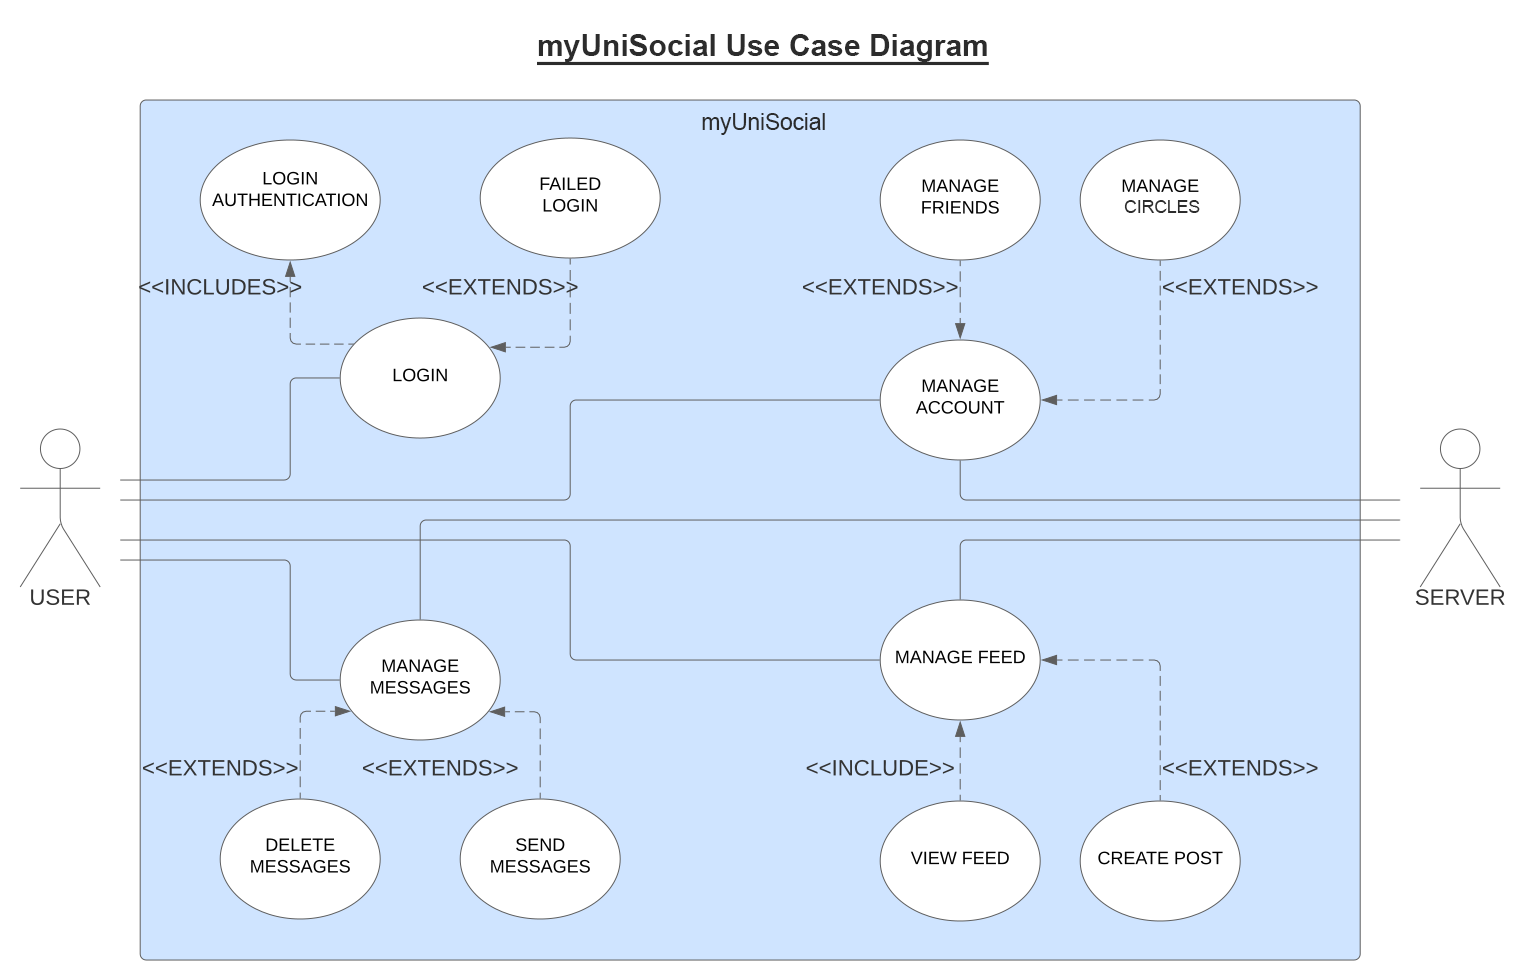
\includegraphics[width=.8\textwidth]{myUniSocialUseCaseDiagram.png}
 	\end{tabular}
\end{figure}
\clearpage

\section{R Studio Testing procedure}
R
\newpage

\section{Ethics Approval}
The following ethics approval form has been submitted.
\begin{table}[h!]
\begin{tabular}{ll}
\hline
\multicolumn{1}{|l|}{\begin{tabular}[c]{@{}l@{}}\\Will your project involve participants?\\ \\
\end{tabular}} & \multicolumn{1}{l|}{Yes} \\ \hline
\multicolumn{1}{|l|}{\begin{tabular}[c]{@{}l@{}}\\Will it be necessary for participants to take part in the
study\\ without their knowledge and consent at the time? (e.g. covert\\ observation of people in non-public places)\\ \\
\end{tabular}} & \multicolumn{1}{l|}{No} \\ \hline
\multicolumn{1}{|l|}{\begin{tabular}[c]{@{}l@{}}\\Will financial inducements (other than reasonable expenses\\ and compensation for time)
be offered to participants?\\ \\
\end{tabular}} & \multicolumn{1}{l|}{No} \\ \hline
\multicolumn{1}{|l|}{\begin{tabular}[c]{@{}l@{}}\\Will your project involve collecting participant data
(e.g.\\ personal and/or sensitive data referring to a living individual)?\\ \\
\end{tabular}} & \multicolumn{1}{l|}{Yes} \\ \hline
\multicolumn{1}{|l|}{\begin{tabular}[c]{@{}l@{}}\\Will your project involve accessing secondary data that is not\\ in the public
domain (e.g. personal data collected by\\ another user)?\\ \\\end{tabular}} & \multicolumn{1}{l|}{Yes} \\ \hline
\multicolumn{1}{|l|}{\begin{tabular}[c]{@{}l@{}}\\Will your project involve accessing commercially sensitive\\ information?\\ \\
\end{tabular}}& \multicolumn{1}{l|}{Yes} \\ \hline
\multicolumn{1}{|l|}{\begin{tabular}[c]{@{}l@{}}\\Could your project have negative environmental impacts\\
(e.g. disturbance of natural habitats; damage to, or contamination\\ of, buildings/artefacts/wildlife)\\ \\
\end{tabular}} & \multicolumn{1}{l|}{No}  \\ \hline
 &
\end{tabular}
\end{table}

The study will be of medium risk, given that none of the high risk criteria applied to this project and that the above stated medium risk elements will
be used at some point within the research and development of myUniSocial.

My project will involve the creation of a social media platform to be used as a learning and socialization tool for universities and higher education institutions.
The methodology for my study will be to conduct a between subjects study involving two study groups. Both groups will be given the same set of tasks to complete, group A will be asked to fulfil these tasks on the existing university platform ie Learning Space or Moodle while group B will be asked to complete them on my prototype platform. 
I will use a survey to collect users experience of both platforms to gauge how much of a benefit they feel the systems to be in both the learning and social sides to university life.




%\section{Biography Section}
%If you have an EPS/PDF photo (graphicx package needed), extra braces are
% needed around the contents of the optional argument to biography to prevent
% the LaTeX parser from getting confused when it sees the complicated
% $\backslash${\tt{includegraphics}} command within an optional argument. (You can create
% your own custom macro containing the $\backslash${\tt{includegraphics}} command to make things
% simpler here.)

\vspace{11pt}

%\bf{If you include a photo:}\vspace{-33pt}
%\begin{IEEEbiography}[{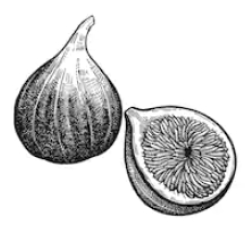
\includegraphics[width=1in,height=1.25in,clip,keepaspectratio]{fig1}}]{Michael Shell}
%Use $\backslash${\tt{begin\{IEEEbiography\}}} and then for the 1st argument use $\backslash${\tt{includegraphics}} to declare and link the author photo.
%Use the author name as the 3rd argument followed by the biography text.
%\end{IEEEbiography}

\vspace{11pt}

%\bf{If you will not include a photo:}\vspace{-33pt}
%\begin{IEEEbiographynophoto}{John Doe}
%Use $\backslash${\tt{begin\{IEEEbiographynophoto\}}} and the author name as the argument followed by the biography text.
%\end{IEEEbiographynophoto}

\vfill
\end{document}
